\documentclass[12pt]{article}
\usepackage{verbatim}
\usepackage[dvips]{epsfig}
\usepackage{color}
\usepackage{url}
\usepackage[colorlinks=true]{hyperref}

\begin{document}

\section*{GENESIS: Documentation}

{\bf Related Documentation:}
% start: userdocs-tag-replace-items related-do-nothing
% end: userdocs-tag-replace-items related-do-nothing

\section*{g-tube Technical Specification}

	This document outlines the design process employed in the development of the {\bf g-tube}, a graphical user interface which brings all components of the {\bf GENESIS3} system together. With the {\bf g-tube} a user can load, create and run models, track all aspects of the simulation including the schedule, parameters, models, underlying software versions, and directly load the output of simulation runs into {\bf Atoms} that can be processed into tables, plots, and formatted text suitable for inserting into manuscripts. The end result of a {\bf g-tube project} will be a compiled electronic publication, containing the finalized document, with all of the data used to generate the figures {\bf tag-associated}  with the model experiment runs. 

\section*{History}

	User interfaces for running simulations have always been difficult to create due to the structure of the simulators they are meant to be used for. The desire for a unified graphical environment for being able to load, run, display output, and save your simulation data has been coveted for quite some time. In GENESIS 2 a model was composed of a series of scripts, which were essentially programs often containing their own logic and flow control. Building a GUI on top of such logic is very difficult as inputs, outputs and internal data structures of the model can all be changed within the logic of the models scripts, thus making it difficult for the GUI logic to track and control all of possible use cases. With the emergence of declarative formats in computational neuroscience, the ability to build interfaces on top of models in a more general way has become more feasible.

\section*{Data Design}

\subsection*{Project Specification}

	A project is a class data structure that is used to track all work done by the user within the {\bf g-tube}. Projects are treated as a combination of categorized lists of data that grow and shrink as the user goes through the {\bf user workflow}. Data tracked includes:
	
\begin{itemize}
	\item[] Project name.
	\item[] List of atoms.
	\item[] Manuscript pages.
	\item[] GUI perspective state.
\end{itemize}

From a file storage perspective a project consists of a directory containing all files in the users workspace along with a {\bf yaml} file that bears the same name as the project. The {\bf yaml} file provides a mapping for all of the files in the project directory so that they can be loaded by the appropriate data management objects within the GUI.

\subsection*{Object Relationships}

	The {\bf g-tube} is set up with a set of "management" classes; their purpose is to provide high level control for the GUI to work with all of the underlying systems, without allowing code from unrelated systems to interlace with one another. This separation allows these complex data management classes to be developed and tested separately.

\begin{itemize}
	\item[] {\bf Project Manager:} Loads or creates a project specification and allows for creating, deleting and editing Model, Atom, Manuscript, and Review management objects.
	\item[] {\bf G3 User Workflow Manager:} Manages a list of models associated with the current project, along with model states and {\bf SSP} configurations.
	\item[] {\bf Simulator Manager:} Manages a registry of simulators to run experiments.
	\item[] {\bf Atom Manager:} Manages a list of all of the atoms in the current project. 
	\item[] {\bf Manuscript Manager:} Manages the atoms tagged as part of a manuscript.
	\item[] {\bf Review Manager:} Manages the compiled manuscript atoms for review.
\end{itemize}


\begin{figure}[ht]
   \centering
   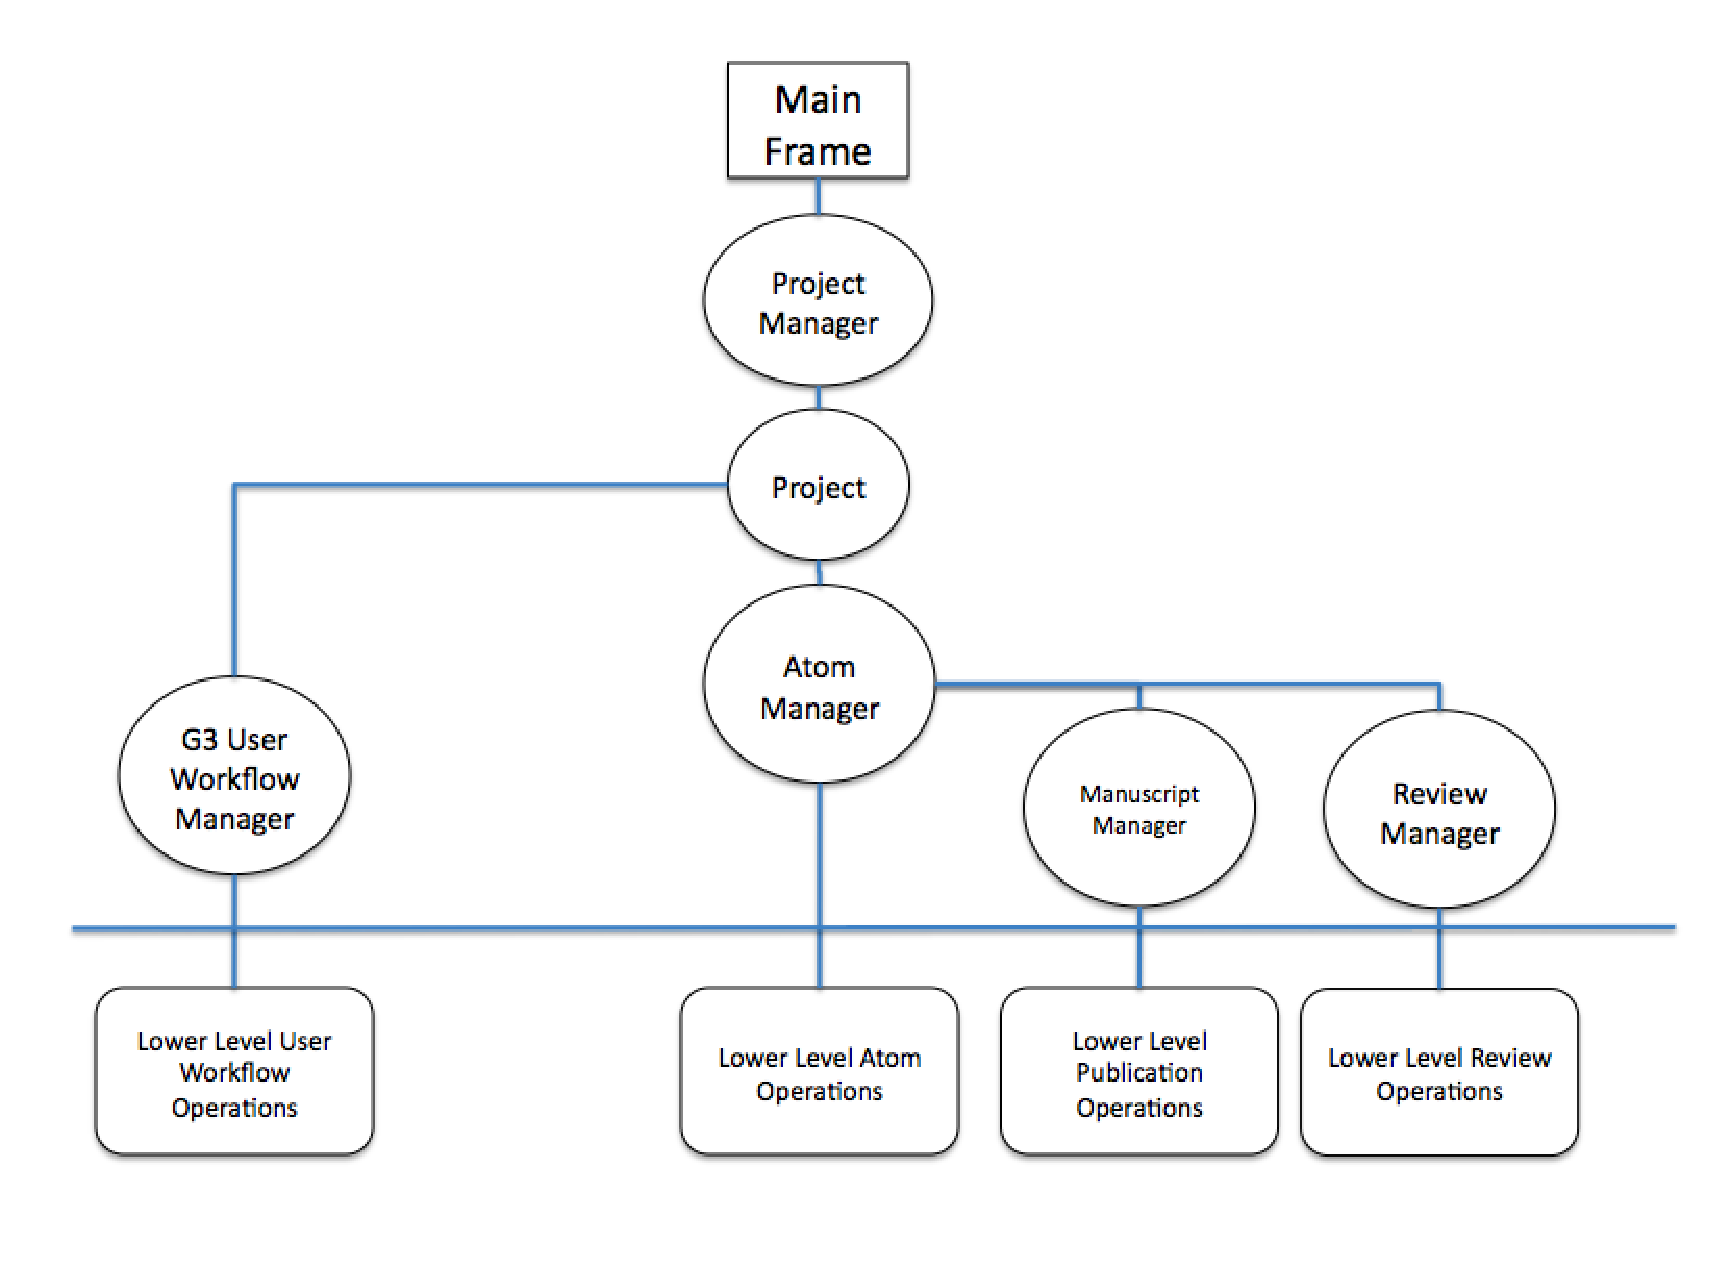
\includegraphics[scale=0.50]{figures/Overview.eps}
   \caption{{\bf Object overview:} A general overview of class relationships within the g-tube.}
   \label{figure: 1}
\end{figure}


The Atom management object allows for basic list operations such as adding, deleting, and editing members. Manuscript and Review managers are subclasses of the Atom manager, that display tag-filtered views of atoms in the project workspace. Management objects encapsulate {\bf wxPython} operations for allowing the end user to perform these actions graphically by drawing their control widgets to the Main Frame. 

\subsection*{Workflow Relationships}

	Due to the nice separation of tasks in the GENESIS user workflow it is easy to disseminate responsibilities amongst higher level management classes.

\begin{figure}[ht]
   \centering
   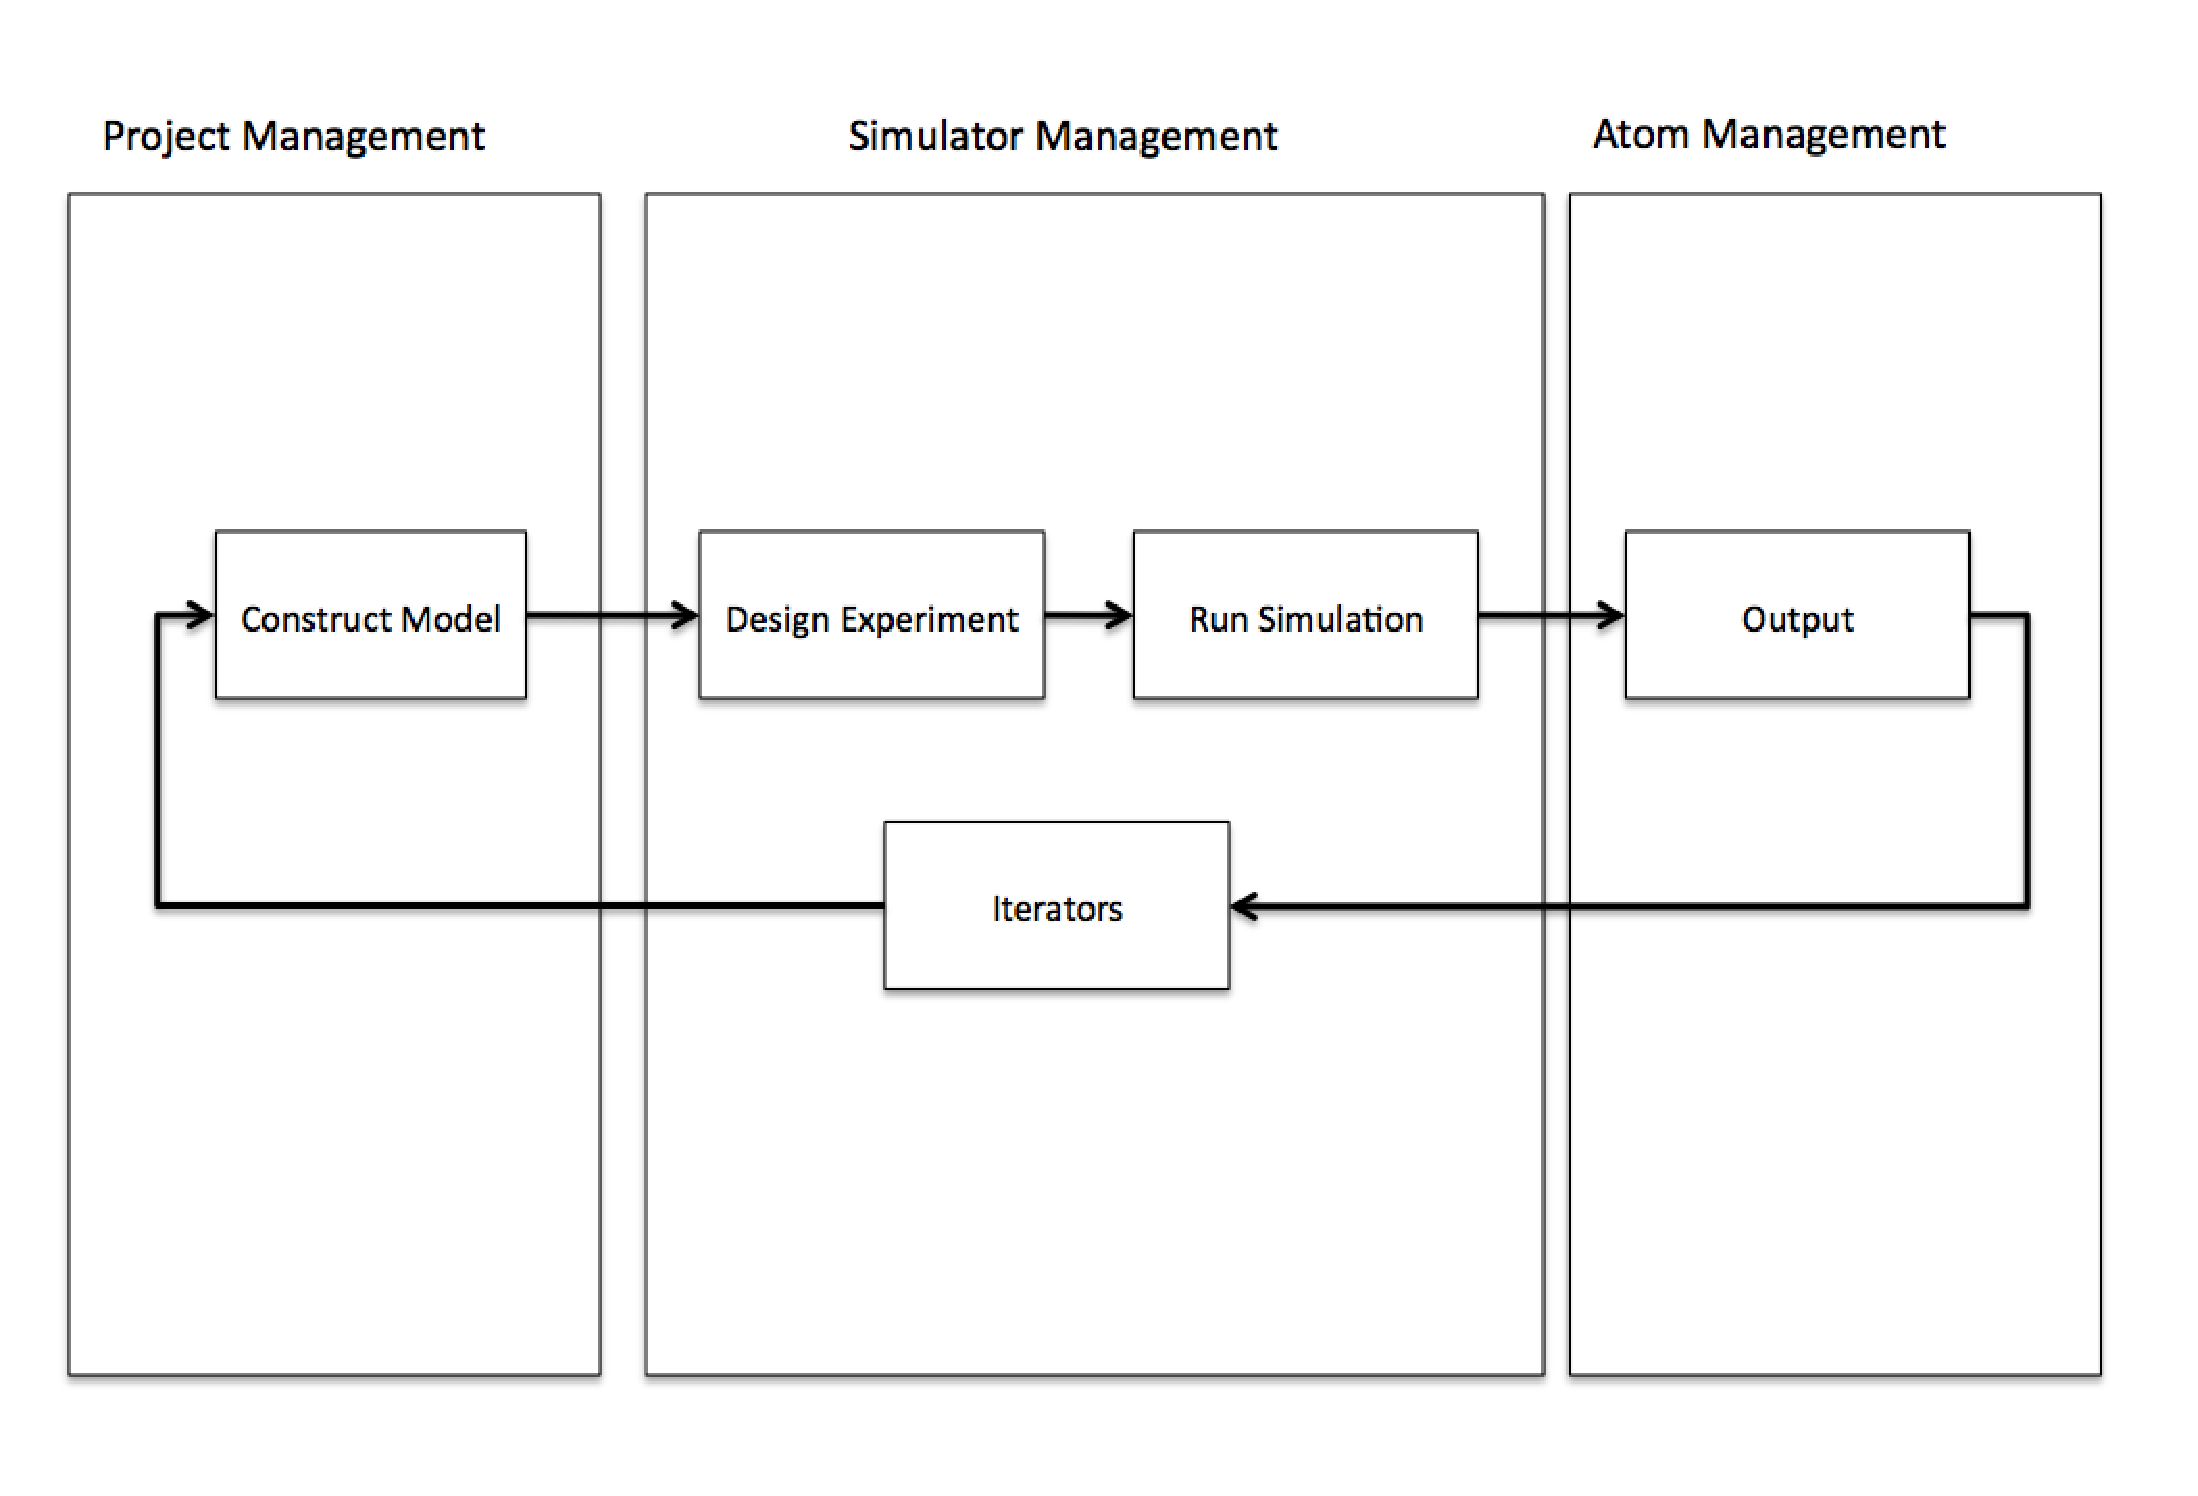
\includegraphics[scale=0.40]{figures/WorkflowSegmentation.eps}
   \caption{{\bf Workflow segmentation:} A figure displaying the separation of responsibilities.}
   \label{figure: 2}
\end{figure}

\subsection*{Model Object}

	To constrain the complexities of interfacing with the whole of the {\bf GENESIS3} system, modeling functionality is isolated to a single class. In principle this should allow other simulators to be encapsulated within the same abstract data type so long it is mapped to the predefined inputs and outputs the {\bf SimulatorManager} uses to communicate with the rest of the system.
	Currently interfacing is done via the {\bf gshell} over file descriptors via the object class called {\it bridge}. 
	
\subsection*{Project Explorer Tabs}

	To navigate the various files the user works with in a project there are four tabs which correspond to each management class. Each tab functionality is categorized as such:
	
\begin{itemize}
\item[] G3 User Workflow
\item[] Content Selection
\item[] Model Validation
\item[] Review Validation
\end{itemize}


\section*{Architecture Design}

\subsubsection*{Plugins}

Due to the unique requirements for some neuroscience projects, some aspects of the software may need to be changed. Since many newer users feel more comfortable using a user interface, allowing the gtube to let users drop in their own implementations can be beneficial. Using the powerful {\bf Python} language the {\bf gtube} will employ a true plugin based system for added extensibility beyond the scope of the initial development. Among attributes that will be extendable are:

\begin{itemize}
\item[] {\bf Simulators}: The gtube is designed to be independent of the underlying simulator (currently GENESIS3), with communication between the presentation layer and functional layer handled via a documented API. Via the API, a developer can make their own simulator compatible with the gtube such that a user familiar with the top level control of the GUI can proceed as normal after selecting a different simulator. The benefits of constraining the control of a simulator to an object are: 

	\begin{itemize}
		\item[] 1. It makes it easy to control from a gui, user interfaces are difficult to manage on simulators due to them being designed to mainly work via the command line.
		\item[] 2. Reducing coupling between objects allows easier debugging and recovery in the event of an error.
		\item[] 3. A well known object API with known entry and exit points is inviting for developers.
	\end{itemize}
		
	
\item[] {\bf Widgets}: One of the main strengths of GENESIS 2 was XODUS, a scriptable user interface where users can build specific guis via scripting and specialized widgets using the X11 library. However adding a new widget to XODUS isn't a job for someone new to programming, and running the newly created widget involved creating a GENESIS 2 script to properly draw it to the screen. To make it easy to add your own widgets, the gtube will employ a plugin system that can dynamically load widgets to a registry, and allow them to be called via the top level gui. 
	Widgets are primarily for displaying data from result files (usually raw text atoms), which are managed by the Atom Manager. Since the Atom Manager allows the user to "tag" any atom from the interface; it is possible for the Atom Manager to match tags to the appropriate widget in the registry and properly display the data. 

\end{itemize}

Below is an example of the levels of abstraction needed to create a usable plugin system for simulator management.

\begin{figure}[ht]
   \centering
   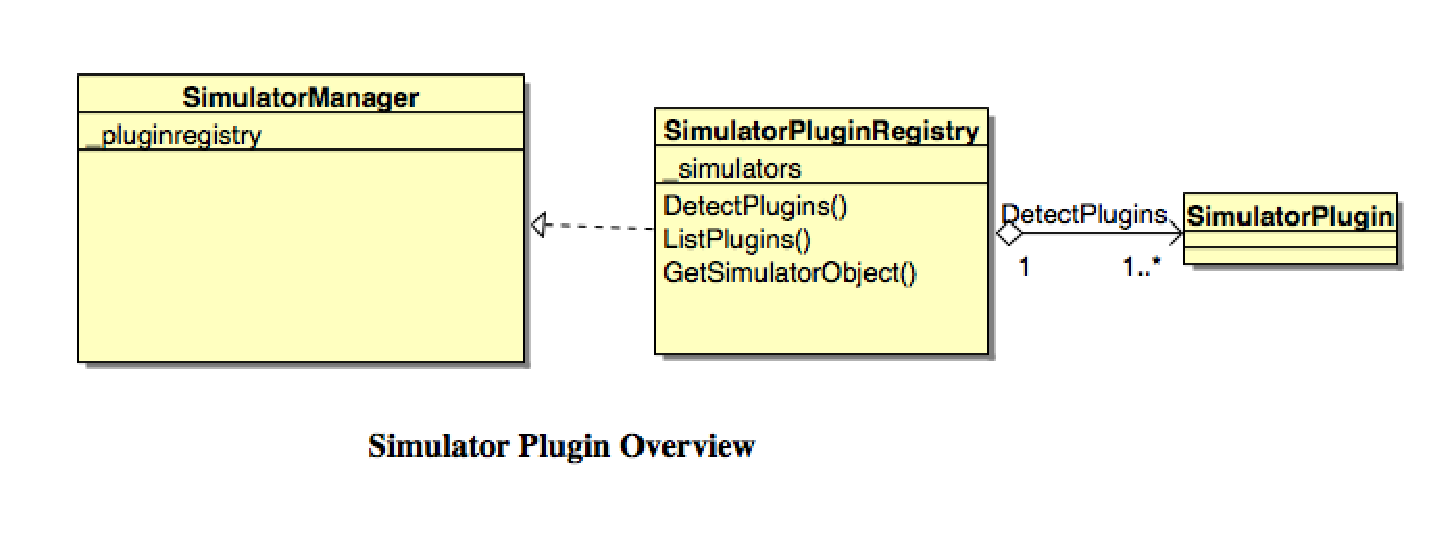
\includegraphics[scale=0.6]{figures/SimulatorPluginOverview.eps}
   \caption{{\bf Simulator Plugins:} Figure shows a UML diagram of the relationships between loadable simulator objects and the Manager class of the GUI logic.}
   \label{fig:Simulator Plugin Overview}
\end{figure}

\subsubsection*{Simulator Object}

	The simulation object is designed with base classes that have functionality directly tied into the user workflow. This allows for a neater separation of code that is specific to their own tasks. The top level of the object contains the operations necessary to start, stop, and detect if the simulator is running. 

\begin{figure}[ht]
   \centering
   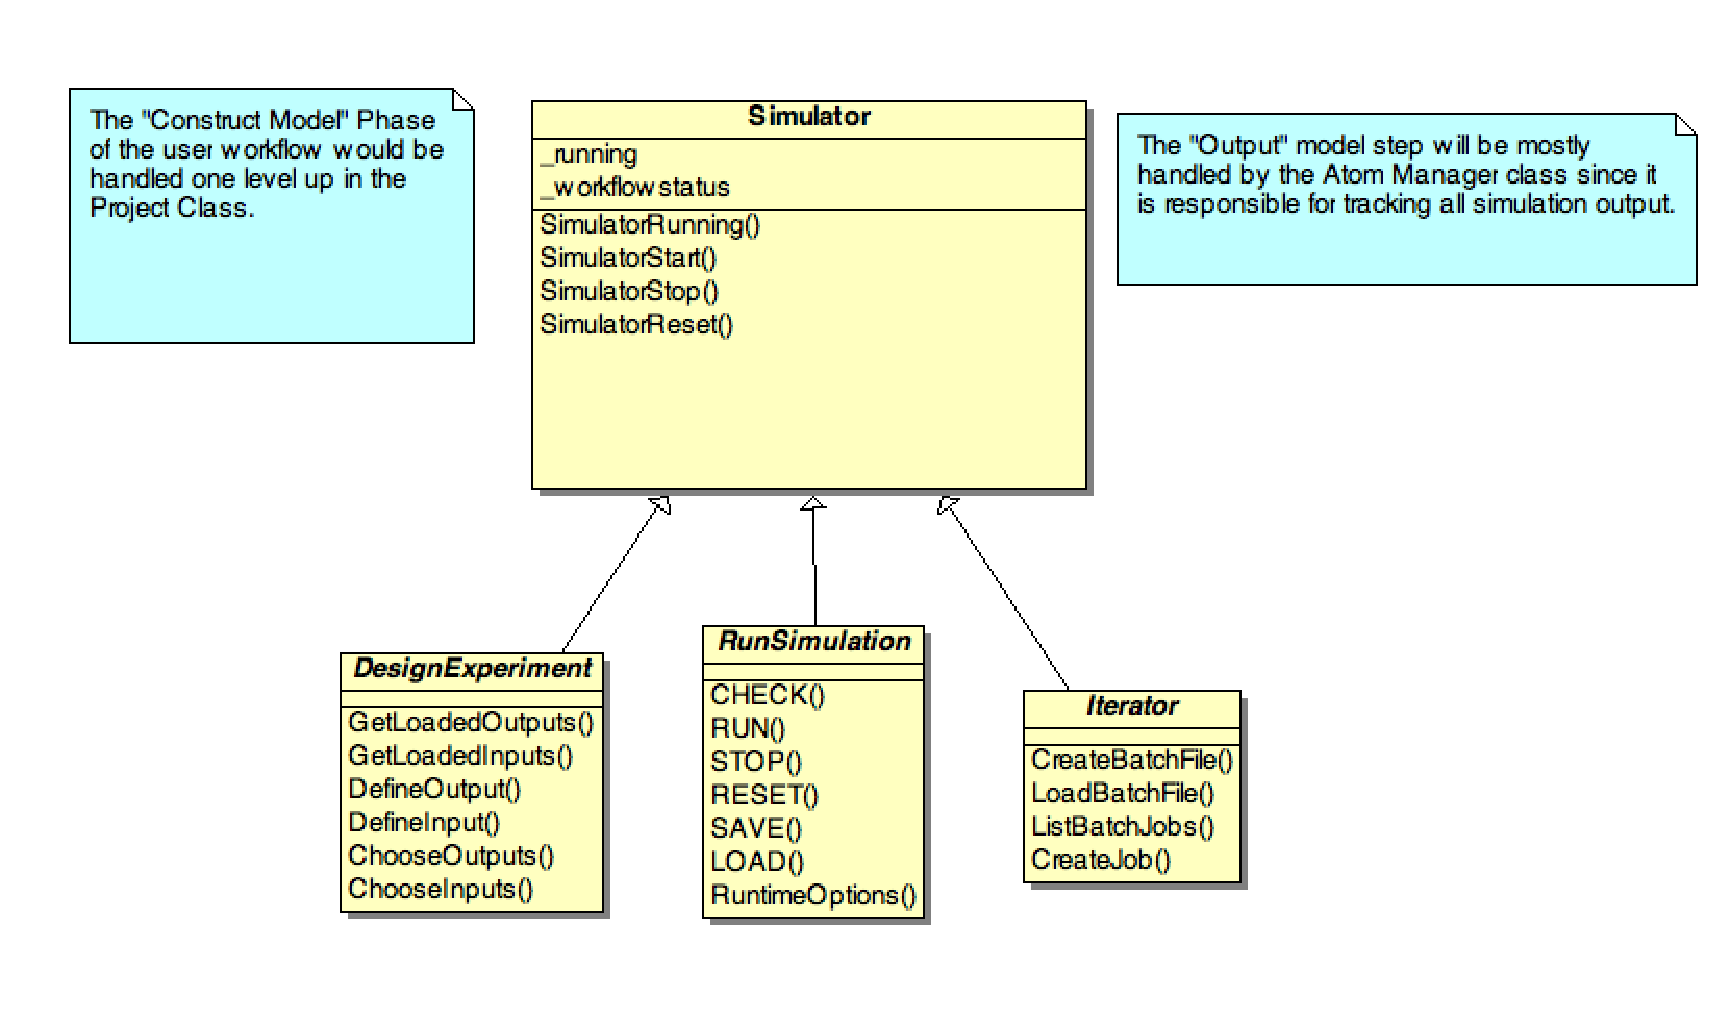
\includegraphics[scale=0.6]{figures/SimulatorObject.eps}
   \caption{{\bf Simulator Object:} Figure shows a UML diagram of the simulator object with it's inherited base classes that directly tie in to the user workflow.}
   \label{fig:Simulator Object}
\end{figure}


\section*{Interface Design}

\subsection*{UI Real Estate}

Presentation of widgets is implemented with the {\bf wxPython} Advanced User Interface (AUI) toolkit. This allows for several dockable panes that the user can rearrange to their liking. 

\begin{figure}[ht]
   \centering
   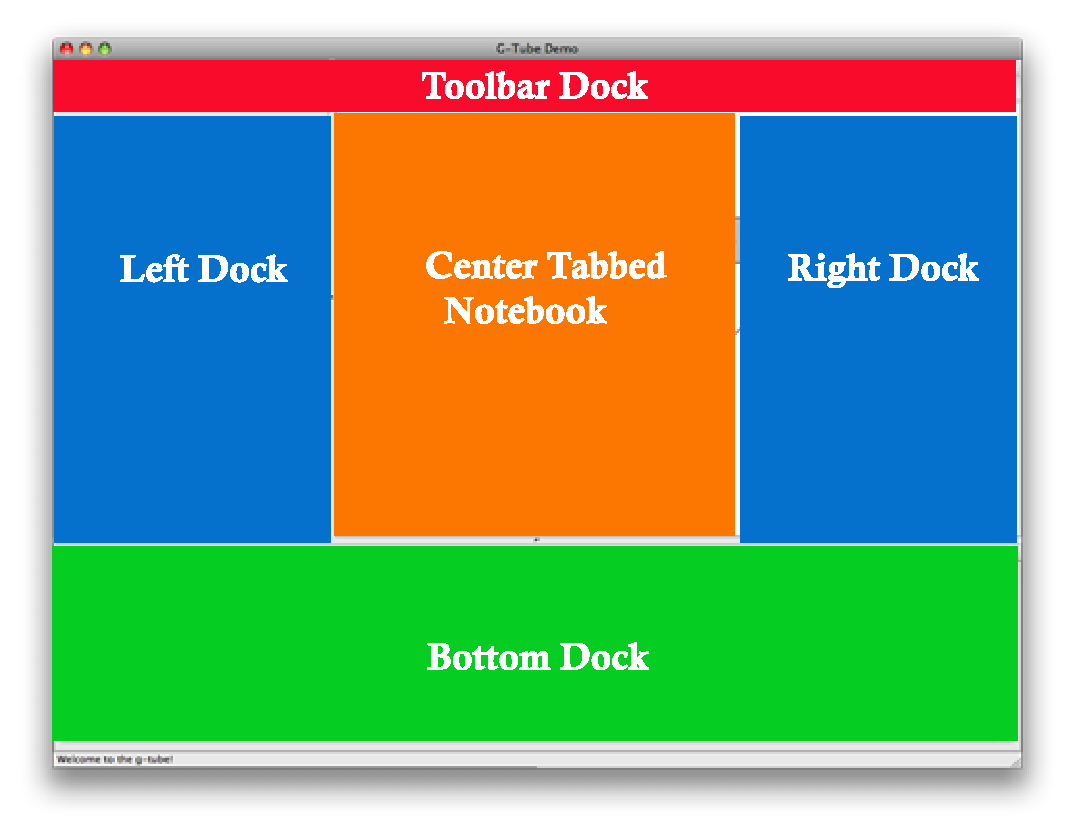
\includegraphics[scale=0.6]{figures/RealEstate.eps}
   \caption{{\bf Main Frame Layout:} Figure shows the default layout of the frames dockable panels.}
   \label{fig:Real Estate}
\end{figure}

\begin{itemize}
\item[] {\bf Toolbar Dock:} Holds icon labeled buttons for performing many shortcuts within the system. Toolbars can be removed from the dock and allows to float at different areas of the screen.
\item[] {\bf Left Dock:} The primary dock for explorer widgets used to manage data in the {\bf Model}, {\bf Atom}, {\bf Manuscript}, and {\bf Review} workspaces.
\item[] {\bf Center Tabbed Notebook:} The "main" workspace. All data selected from a workspace via an explorer will be displayed in a Tab in the Center Notebook. E.G Editable Documents, Manuscript Atoms, Plots from simulation.
\item[] {\bf Right Dock:} Primarily used to hold widgets for editing attributes (such as tags) to the current working tab in the Center Notebook.
\item[] {\bf Bottom Dock:} Primarily holds widgets that output data from the underlying system. E.G Console output from the {\bf g-tube}, model status, error messages.
\end{itemize}

\section*{Procedural Design}

\subsection*{Development Tools}

	The implementation of the {\bf g-tube} is done in {\bf Python} using the {\bf wxPython} widget toolkit. The {\bf wxPython} toolkit is a Python extension module of the popular {wxWidgets} coss-platform GUI library. This allows the user to create widgets with the look and feel of the host operating system while using the powerful {\bf Python} language. {\bf wxPython} is open source, has many contributors, boasts a large collection of example tutorials and documentation, and possesses one of the friendliest communities. 


The following {\bf Python} dependencies are also required:

\begin{itemize}	
\item[] {\bf yaml:} For parsing and loading configuration and data files.
\item[] {\bf matplotlib:} Provides more refined plot panels.
\item[] {\bf PyOpenGL:} Required for 3D graphics. Available \href{http://pyopengl.sourceforge.net/}{here.}
\end{itemize}

Higher level GUI construction is done using \href{http://xrced.sourceforge.net/}{\bf XRCed}, a simple graphical editor that creates Python classes with embedded (or externally loaded) \href{http://wiki.wxpython.org/XRCTutorial}{\bf XRC} files. 


\subsection*{Coding Style}
	To ensure maximum compatibility across different versions of python, coding will follow the {\bf Python} Code \href{http://www.python.org/dev/peps/pep-0008/}{Style Guide} with the exception of using camel case for module names, a convention inherited from wxPython. 
	
\subsubsection*{Private members}	
	Python does not have any truly private members within classes, so prefixing with "\_" is used for weak privatizing of operations or attributes, and "\_\_" is used for strong privatizing (also called "name mangling"). Example:
	
\begin{verbatim}
	class foo:

	  def __init__(self,value):

	    self.__my_value = value

	  # top level methods

	  def pub_get_value(self):
	    return self.__priv_get_value()

	  # private methods

	  def __priv_get_value(self):
	    return self.__my_value

	if __name__ == '__main__':

	  bar = foo(21)

	  print "My value is %s\n" % bar.pub_get_value()
\end{verbatim}

The result of this script is "My value is 21". The value is set to a private internal variable {\it \_\_my\_value}. The public method {\it pub\_get\_value} calls the private method {\it \_\_priv\_get\_variable())} to retrieve the value. A direct call to {\it \_\_priv\_get\_value(} like this:

\begin{verbatim}
	if __name__ == '__main__':

	  bar = foo(21)

	  print "My value is %s\n" % bar.__priv_get_value()
\end{verbatim}

 will produce an error. If the private function was declared with weak privatizing using a single underscore like,  {\it \_priv\_get\_value()}, then it would be possible to call it from the main as follows:

\begin{verbatim}
	if __name__ == '__main__':

	  bar = foo(21)

	  print "My value is %s\n" % bar._priv_get_value()
\end{verbatim}

Privatizing was typically considered "Unpythonic," however due to potential program breaking name conflicts which can occur during inheritance, it is common to privatize methods that are not to be overridden. The {\bf gtube}, being a program that makes use of many object relationships, uses private members where appropriate.


\subsubsection*{Engineering Tools}

For UML and other software figure drawing a "project" directory has been placed in the top level source code directory. In this directory there are project files for:

\begin{itemize}
\item[] \href{http://bouml.free.fr}{\bf bouml}: A freeware cross platform UML diagramming software. It features a wealth of user \href{http://bouml.free.fr/doc/index.html}{documentation} and can export Python code from your diagrams. {\bf Bouml} is also available via apt-get on debian and ubuntu systems. It should be noted that bouml is very unforgiving in it's backward compatability, so any version less than 4.22.2 will not load the versioned project in the repository.
\item[] \href{http://www.stack.nl/~dimitri/doxygen/}{\bf Doxygen}: Doxygen has a UML option that creates very nice looking diagrams with browsable code. An example of how to use Doxygen to document Python code can be found \href{https://www.cells.es/Members/srubio/howto/doxygen/}{\bf here}.
\end{itemize}

As the project increases in scope and size, engineering tools such as this help to keep the project manageable, especially for programmers wishing to modify existing code.




\end{document}
